\documentclass[../main.tex]{subfiles}

\begin{document}

\part{Linear Systems}
\addcontentsline{toc}{section}{Roots and Optimization}

\section[OVERVIEW]{OVERVIEW}
\noindent \textbf{What Are Linear Algebraic Equations?}\\

In Part Two, we determined the value $x$ that satisfied a single equation, $f(x)=0$. Now, we deal with the case of determining the values $x_{1}, x_{2}, \ldots, x_{n}$ that simultaneously satisfy a set of equations:
$$
\begin{gathered}
f_{1}\left(x_{1}, x_{2}, \ldots, x_{n}\right)=0 \\
f_{2}\left(x_{1}, x_{2}, \ldots, x_{n}\right)=0 \\
\vdots \\
f_{n}\left(x_{1}, x_{2}, \ldots, x_{n}\right)=0
\end{gathered}
$$
Such systems are either linear or nonlinear. In Part Three, we deal with linear algebraic equations that are of the general form

$$
\begin{gathered}
a_{11} x_{1}+a_{12} x_{2}+\cdots+a_{1 n} x_{n}=b_{1} \\
a_{21} x_{1}+a_{22} x_{2}+\cdots+a_{2 n} x_{n}=b_{2} \\
\vdots \\
\vdots \\
a_{n 1} x_{1}+a_{n 2} x_{2}+\cdots+a_{n n} x_{n}=b_{n}
\end{gathered}
$$
where the $a$ 's are constant coefficients, the $b$ 's are constants, the $x$ 's are unknowns, and $n$ is the number of equations. All other algebraic equations are nonlinear.
\\

\noindent \textbf{Linear Algebraic Equations in Engineering and Science}\\

Many of the fundamental equations of engineering and science are based on conservation laws. Some familiar quantities that conform to such laws are mass, energy, and momentum. In mathematical terms, these principles lead to balance or continuity equations that relate system behavior as represented

\begin{center}
    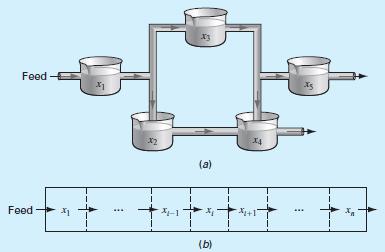
\includegraphics[width=0.6\linewidth]{./images/fig_PT3_1}

    \textsf{FIGURE PT3.1 - Two types of systems that can be modeled using linear algebraic equations: (a) lumped variable
    system that involves coupled finite components and (b) distributed variable system that involves
    a continuum.}
\end{center}

\noindent by the levels or response of the quantity being modeled to the properties or characteristics of the system and the external stimuli or forcing functions acting on the system.

As an example, the principle of mass conservation can be used to formulate a model for a series of chemical reactors (Fig. PT3.1a). For this case, the quantity being modeled is the mass of the chemical in each reactor. The system properties are the reaction characteristics of the chemical and the reactors' sizes and flow rates. The forcing functions are the feed rates of the chemical into the system.

When we studied roots of equations, you saw how single-component systems result in a single equation that can be solved using root-location techniques. Multicomponent systems result in a coupled set of mathematical equations that must be solved simultaneously. The equations are coupled because the individual parts of the system are influenced by other parts. For example, in Fig. PT3.1a, reactor 4 receives chemical inputs from reactors 2 and 3 . Consequently, its response is dependent on the quantity of chemical in these other reactors.
When these dependencies are expressed mathematically, the resulting equations are often of the linear algebraic form of Eq. (PT3.1). The $x$ 's are usually measures of the magnitudes of the responses of the individual components. Using Fig. PT3.1 $a$ as an example, $x_{1}$ might quantify the amount of chemical mass in the first reactor, $x_{2}$ might quantify the amount in the second, and so forth. The $a$ 's typically represent the properties and characteristics that bear on the interactions between components. For instance, the $a$ 's for Fig. PT3. la might be reflective of the flow rates of mass between the reactors. Finally, the $b$ 's usually represent the forcing functions acting on the system, such as the feed rate.

Multicomponent problems of these types arise from both lumped (macro-) or distributed (micro-) variable mathematical models. Lumped variable problems involve coupled

finite components. The three interconnected bungee jumpers described at the beginning of Chap. 8 are a lumped system. Other examples include trusses, reactors, and electric circuits.

Conversely, distributed variable problems attempt to describe the spatial detail on a continuous or semicontinuous basis. The distribution of chemicals along the length of an elongated, rectangular reactor (Fig. PT3.1b) is an example of a continuous variable model. Differential equations derived from conservation laws specify the distribution of the dependent variable for such systems. These differential equations can be solved numerically by converting them to an equivalent system of simultaneous algebraic equations.

The solution of such sets of equations represents a major application area for the methods in the following chapters. These equations are coupled because the variables at one location are dependent on the variables in adjoining regions. For example, the concentration at the middle of the reactor in Fig. PT3.1 $b$ is a function of the concentration in adjoining regions. Similar examples could be developed for the spatial distribution of temperature, momentum, or electricity.

Aside from physical systems, simultaneous linear algebraic equations also arise in a variety of mathematical problem contexts. These result when mathematical functions are required to satisfy several conditions simultaneously. Each condition results in an equation that contains known coefficients and unknown variables. The techniques discussed in this part can be used to solve for the unknowns when the equations are linear and algebraic. Some widely used numerical techniques that employ simultaneous equations are regression analysis and spline interpolation.

\bigskip

\section[PART ORGANIZATION]{PART ORGANIZATION}

\noindent
Due to its importance in formulating and solving linear algebraic equations, Chap. 8 provides a brief overview of matrix algebra. Aside from covering the rudiments of matrix representation and manipulation, the chapter also describes how matrices are handled in MATLAB.

Chapter 9 is devoted to the most fundamental technique for solving linear algebraic systems: Gauss elimination. Before launching into a detailed discussion of this technique, a preliminary section deals with simple methods for solving small systems. These approaches are presented to provide you with visual insight and because one of the methodsthe elimination of unknowns-represents the basis for Gauss elimination.

After this preliminary material, "naive" Gauss elimination is discussed. We start with this "stripped-down" version because it allows the fundamental technique to be elaborated on without complicating details. Then, in subsequent sections, we discuss potential problems of the naive approach and present a number of modifications to minimize and circumvent these problems. The focus of this discussion will be the process of switching rows, or partial pivoting. The chapter ends with a brief description of efficient methods for solving tridiagonal matrices.

Chapter 10 illustrates how Gauss elimination can be formulated as an LU factorization. Such solution techniques are valuable for cases where many right-hand-side vectors need to be evaluated. The chapter ends with a brief outline of how MATLAB solves linear systems.

Chapter 11 starts with a description of how $L U$ factorization can be employed to efficiently calculate the matrix inverse, which has tremendous utility in analyzing stimulusresponse relationships of physical systems. The remainder of the chapter is devoted to the important concept of matrix condition. The condition number is introduced as a measure of the roundoff errors that can result when solving ill-conditioned matrices.

Chapter 12 deals with iterative solution techniques, which are similar in spirit to the approximate methods for roots of equations discussed in Chap. 6. That is, they involve guessing a solution and then iterating to obtain a refined estimate. The emphasis is on the GaussSeidel method, although a description is provided of an alternative approach, the Jacobi method. The chapter ends with a brief description of how nonlinear simultaneous equations can be solved.

Finally, Chap. 13 is devoted to eigenvalue problems. These have general mathematical relevance as well as many applications in engineering and science. We describe two simple methods as well as MATLAB's capabilities for determining eigenvalues and eigenvectors. In terms of applications, we focus on their use to study the vibrations and oscillations of mechanical systems and structures.

\end{document}